\chapter{Nexys4-borden gebruiken als een MEGA65}

\section{Uw eigen MEGA65-compatibele computer bouwen}

U kunt uw eigen MEGA65-compatibele computer bouwen met een Nexys4DDR-bord (ook wel Nexys A7) of een ouder Nexys4-bord (zonder DDR).
Deze bijlage beschrijft het proces om een Nexys4DDR (Nexys A7)-bord hiervoor in te stellen (het nieuwere, bij voorkeur te gebruiken bord).
Het oudere non-DDR Nexys4-bord wordt ook ondersteund en de instructies zijn hetzelfde, met uitzondering van het feit dat u een bitstream moet gebruiken die voor dat bord ontworpen is.
Het gebruik van een Nexys4DDR-bitstream op een non-DDR Nexys4-bord of andersom kan onherstelbare schade aan uw bord veroorzaken. Zorg er daarom voor dat u de juiste bitstream voor uw bord heeft.


DISCLAIMER: M.E.G.A kan geen enkele verantwoordelijkheid aanvaarden voor schade die aan uw Nexys4DDR/NexysA7/Nexys4-borden kan ontstaan.

\newpage

\section{Werkende Nexys4-borden}

Er zijn momenteel drie Nexys FPGA-borden die als MEGA65 ingesteld kunnen worden:

\begin{minipage}{\linewidth}
  \subsection{Het Nexys4-bord}

  Niet meer geproduceerd, maar nog wel verkrijgbaar via sommige websites met oude voorraad.

  \begin{center}
    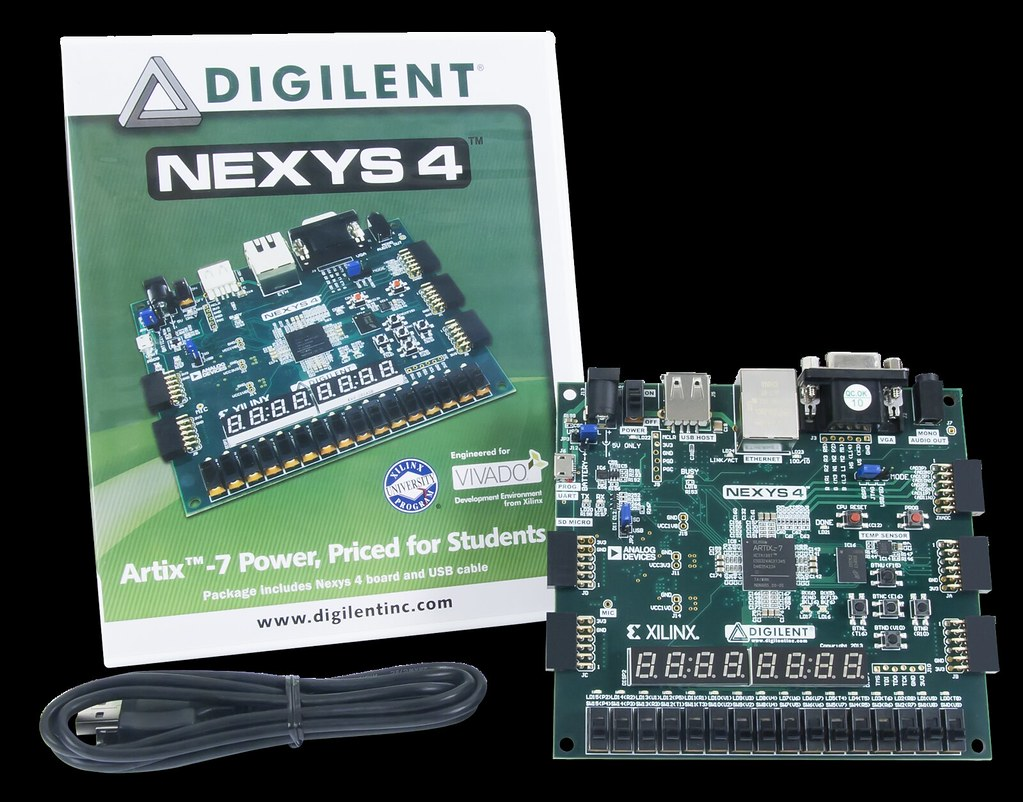
\includegraphics[width=0.4\linewidth]{images/img001_nexys4_board.jpg}
  \end{center}

  Documentatie:

  \begin{itemize}
    \item \url{https://reference.digilentinc.com/reference/programmable-logic/nexys-4/reference-manual}
    \item \url{https://reference.digilentinc.com/\_media/reference/programmable-logic/nexys-4/nexys4\_rm.pdf}
  \end{itemize}
\end{minipage}

\begin{minipage}{\linewidth}
  \subsection{Het Nexys4DDR-bord}

  Niet meer geproduceerd, maar nog wel verkrijgbaar via sommige websites met oude voorraad.

  \begin{center}
    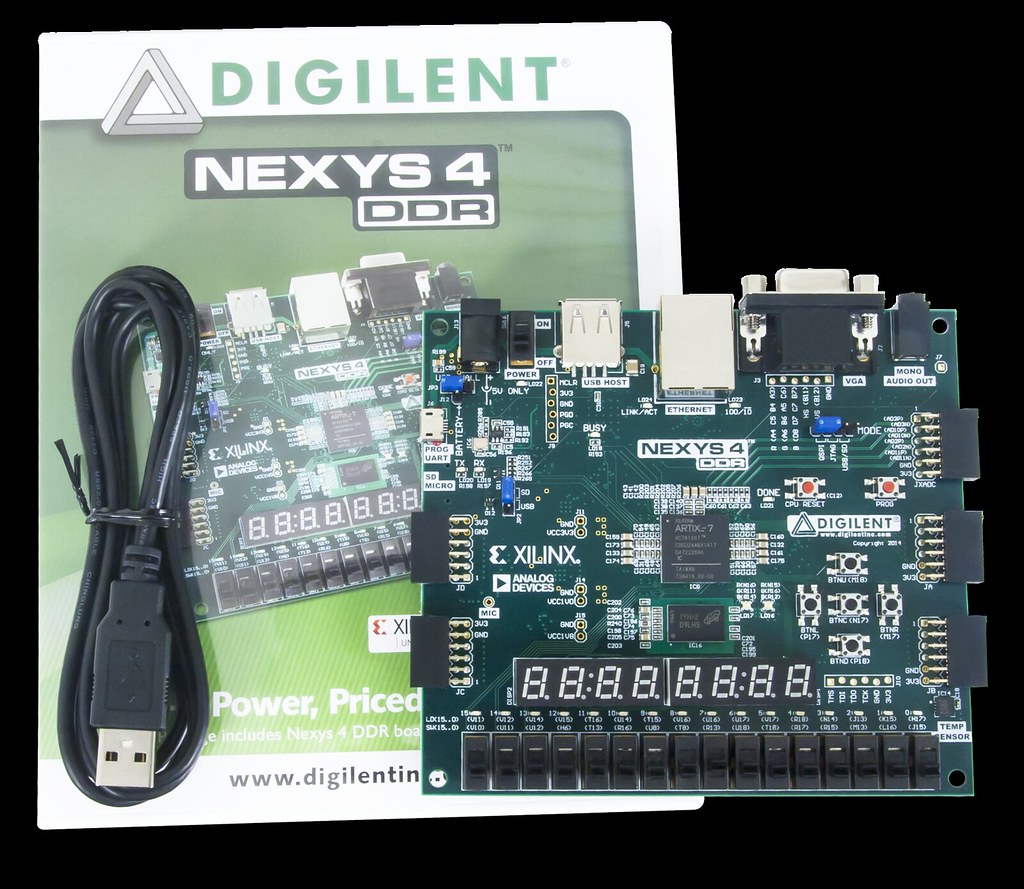
\includegraphics[width=0.4\linewidth]{images/img002_nexys4_ddr_board.jpg}
  \end{center}

  Documentatie:

  \begin{itemize}
    \item \url{https://reference.digilentinc.com/reference/programmable-logic/nexys-4-ddr/reference-manual}
    \item \url{https://reference.digilentinc.com/\_media/reference/programmable-logic/nexys-4-ddr/nexys4ddr\_rm.pdf}
  \end{itemize}
\end{minipage}

\begin{minipage}{\linewidth}
  \subsection{De Nexys A7}

  Dit is het bovenstaande Nexys4 DDR-bord, opnieuw uitgebracht onder een andere naam:

  \begin{center}
    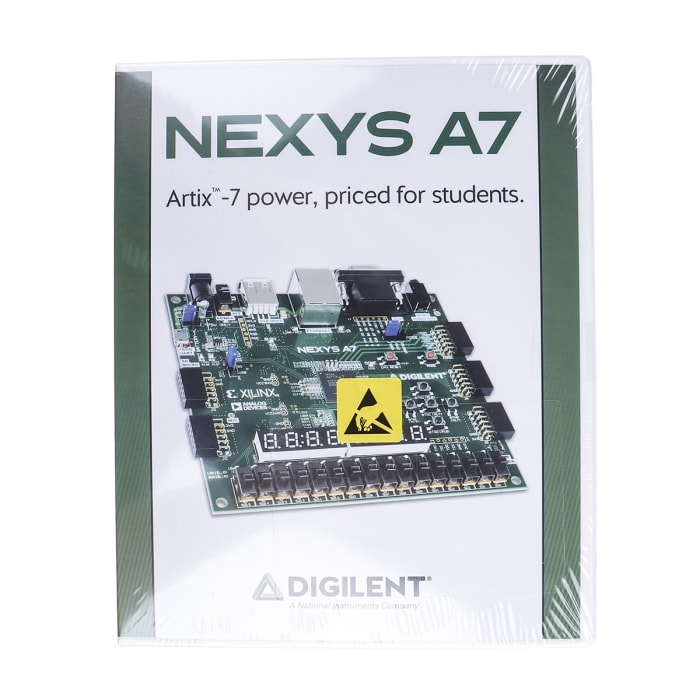
\includegraphics[width=0.4\linewidth]{images/img003_nexysA7_board.jpg}
  \end{center}

  Documentatie:

  \begin{itemize}
    \item \url{https://reference.digilentinc.com/reference/programmable-logic/nexys-a7/reference-manual}
    \item \url{https://reference.digilentinc.com/\_media/reference/programmable-logic/nexys-a7/nexys-a7\_rm.pdf}
  \end{itemize}
\end{minipage}

\newpage

\section{Stroom, jumpers, schakelaars en knoppen}

Deze foto van bovenaf toont de belangrijkste jumperposities op het Nexys4-bord:

  \begin{center}
    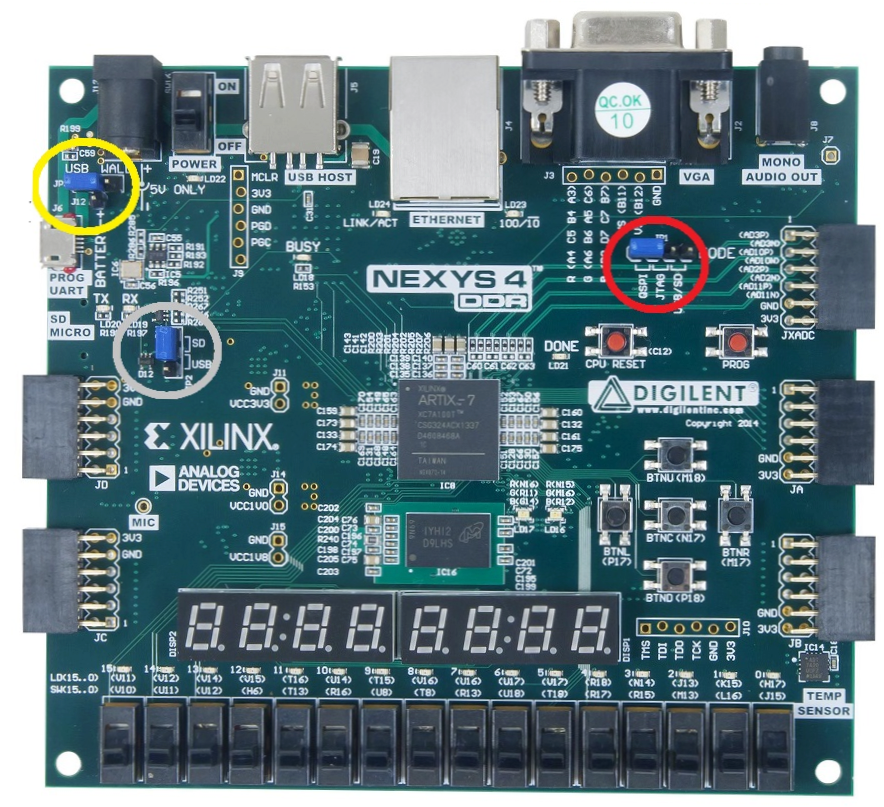
\includegraphics[width=0.9\linewidth]{images/nexys4_jumpers.png}
  \end{center}

De Nexys4-borden kunnen op twee manieren van stroom worden voorzien: via een externe voeding of via een standaard USB-poort.

\subsection{Micro-USB-voeding}

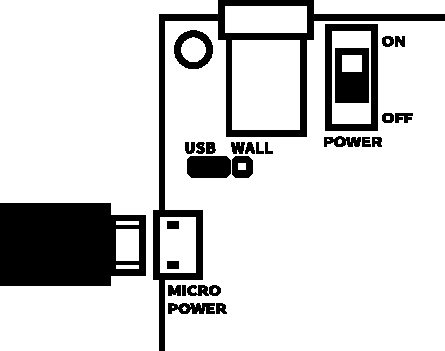
\includegraphics[width=5cm]{images/illustrations/nexys-micro-usb-power.pdf}

Sluit uw micro-USB-kabel aan op een USB-poort van een USB-lader of pc om stroom te leveren. Sluit het andere uiteinde aan op de micro-USB-connector van de Nexys4. Plaats de JP3-jumper op pennen 1 en 2 om USB-voeding te selecteren. Gebruik de schakelaar om de Nexys4 in te schakelen.

\subsection{Externe voeding}

\hspace*{1.7cm}
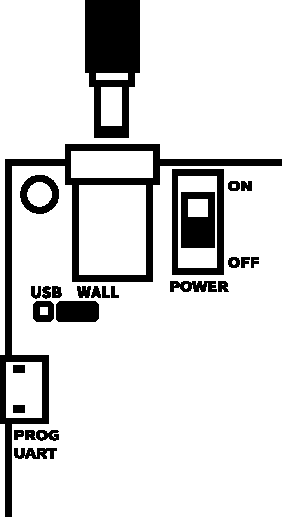
\includegraphics[width=3.2cm]{images/illustrations/nexys-power-supply.pdf}

De MEGA65-core kan veel stroom verbruiken en een standaard USB-poort kan in potentie te weinig vermogen leveren voor het Nexys4-bord. Het schrijven naar de SD-kaart kan met name vastlopen of vreemd gedrag vertonen. U wordt dan aangeraden een voeding van 5V te gebruiken.

Digilent verkoopt een voeding voor het Nexys4-bord en wij raden u aan deze te gebruiken om het risico op schade aan uw Nexys4-bord te vermijden. De gekozen voeding moet een center-positieve stekker met een binnendiameter van 2.1 mm hebben en 4.5VDC tot 5.5VDC leveren met een stroomsterkte van ten minste 1 ampère.

Sluit de voedingskabel aan op de voedingsaansluiting van de Nexys4. Plaats de JP3-jumper op pennen 2 en 3 om netvoeding te selecteren. Gebruik de schakelaar om de Nexys4 in te schakelen.

\subsection{Overige jumpers en schakelaars}

Voor uw eerste installatie raden wij u aan de volgende jumpers op uw Nexys4-bord in te stellen:

\begin{itemize}
  \item{JP1} - USB/SD  \item{JP2} - SD
\end{itemize}

\begin{center}
  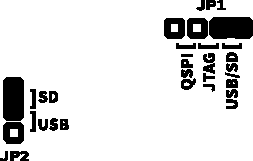
\includegraphics[width=3.2cm]{images/illustrations/nexys-jumpers.pdf}
\end{center}

Dit zorgt ervoor dat de bitstream-bestanden bij het opstarten vanaf uw SD-kaart geladen worden.

Op een later moment kunt u ervoor kiezen de bitstream vanaf de ingebouwde QSPI-flash te laden. In dat geval kunt u de instelling van de JP1-jumper aanpassen naar de QSPI-positie.

% XXX - Image of board highlighting the jumpers

Alle 16 schakelaars aan de onderkant van het bord moeten op de uit-positie staan.


\subsection{Aansluitingen en randapparatuur}

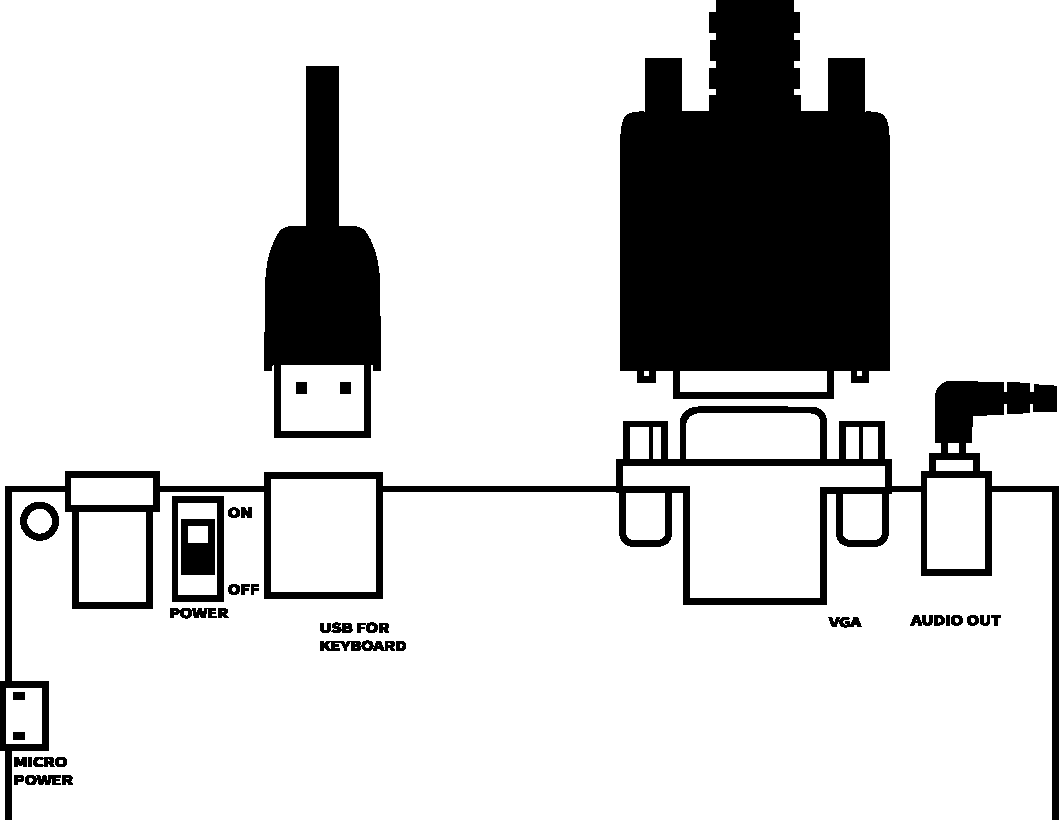
\includegraphics[width=\linewidth]{images/illustrations/nexys-connectors.pdf}

Aan de USB-poort kan een USB-toetsenbord worden aangesloten. Alleen een toetsenbord zonder USB-hub werkt met het Nexys4-bord. Over het algemeen werken zeer goedkope toetsenborden, terwijl duurdere toetsenborden vaak een USB-hub bevatten en niet werken. Het zou kunnen voorkomen dat u meerdere toetsenborden moet proberen voordat u er een vindt die werkt.

Aan de VGA-poort kan een VGA-beeldscherm worden aangesloten.

De mono-audio-uitgang kan worden aangesloten op de line-in van een versterker.


\subsection{Communicatie met uw pc}

Er kunnen situaties zijn waarin u vanaf uw pc met het Nexys4-bord wilt communiceren, bijvoorbeeld om de volgende activiteiten uit te voeren:

\begin{itemize}
  \item Het QSPI-flashgeheugen flashen via Vivado  \item Bitstream-bestanden rechtstreeks vanaf uw pc uploaden (via het m65-hulpprogramma)  \item Hulpprogramma's gebruiken zoals M65Connect, m65, mega65\_ftp, m65dbg, enz.
\end{itemize}

In zulke gevallen moet u de micro-USB-kabel op uw pc aansluiten.

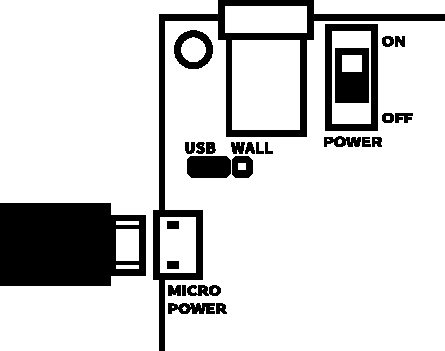
\includegraphics[width=5cm]{images/illustrations/nexys-micro-usb-power.pdf}

\subsection{Knoppen op het bord}

\begin{center}
  
\includegraphics[width=3.2cm]{images/illustrations/nexys-reset-buttons.pdf}
\end{center}

De ``CPU RESET''-toets reset de MEGA65 wanneer u deze indrukt, terwijl de ``PROG''-toets de FPGA zelf de MEGA65-core laat herladen. Het belangrijkste verschil tussen de twee is dat CPU RESET sneller is en de inhoud van het geheugen niet wist, terwijl de FPGA-knop langzamer is en de inhoud van het geheugen wel reset.

\begin{center}
  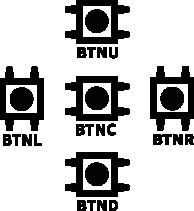
\includegraphics[width=3.2cm]{images/illustrations/nexys-five-buttons.pdf}
\end{center}

Twee van de vijf toetsen in de kruisopstelling kunnen eveneens worden gebruikt: BTND gedraagt zich alsof u \widekey{RESTORE} heeft ingedrukt, terwijl BTNC een interrupt activeert, alsof de IRQ-lijn naar massa is getrokken.

\section{Toetsenbord}

De toetsenbordindeling is positioneel en niet logisch. Dit betekent dat toetsen die zich in dezelfde positie bevinden als de toetsen op een C65-toetsenbord een vergelijkbare functie hebben. Deze relatie gaat ervan uit dat uw USB-toetsenbord een Amerikaanse toetsenbordindeling gebruikt.

Om u te helpen bij het vinden van de toetstoewijzingen van de diverse MEGA65-toetsen, beschikt de MEGA65 over een ingebouwde virtuele toetsenbordtest. Deze is op twee manieren te bereiken.

De eenvoudigste manier is om \specialkey{ALT} ingedrukt te houden terwijl u de Nexys4 inschakelt, of de Nexys4 reset met de ``PROG''-toets. Het configuratiemenu wordt weergegeven en door op 3 te drukken, verschijnt het virtuele toetsenbord op een zwarte achtergrond.

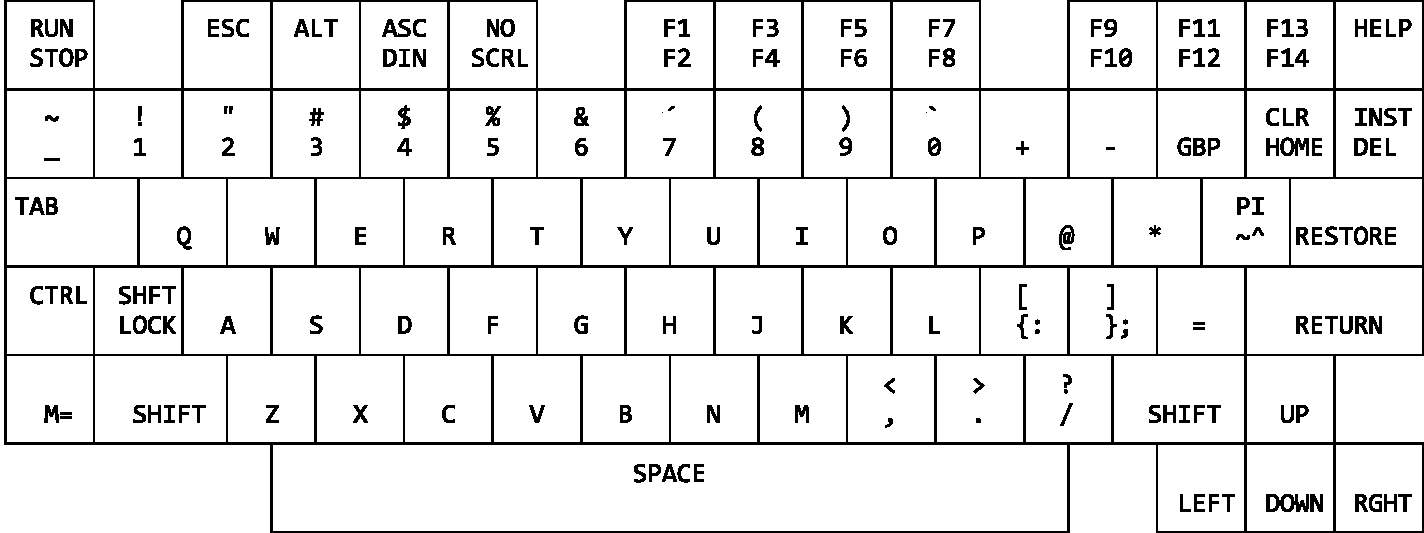
\includegraphics[width=\linewidth]{images/illustrations/virtual-keyboard.pdf}

Wanneer u een toets op het USB-toetsenbord indrukt, wordt de betreffende toets op het virtuele toetsenbord gemarkeerd weergegeven om u te helpen bij het herkennen van de toetstoewijzing.

De andere manier om het virtuele toetsenbord te bereiken is vanuit de MEGA65 zelf. Houd \megasymbolkey ingedrukt en druk op \specialkey{TAB} om de Matrix Mode Debugger te openen. Voer vervolgens het volgende in:

\screentextwide{s ffd3615 ff}

Dit opent een halfdoorzichtig virtueel toetsenbord aan de bovenkant van het scherm. Als alternatief:

\screentextwide{s ffd3615 ff ff}

Dit opent een halfdoorzichtig virtueel toetsenbord in het midden van het scherm.

Houd \megasymbolkey ingedrukt en druk op \specialkey{TAB} om de Matrix Mode Debugger te verlaten en terug te keren naar de MEGA65.

\subsection{Enkele toetstoewijzingen met een USB-toetsenbord}

\widekey{RESTORE} is toegewezen aan de Page Up-toets.

\specialkey{RUN\\STOP} is toegewezen aan \specialkey{ESC}.

\newpage

\section{MicroSDHC-kaart voorbereiden}

De MEGA65 vereist een SDHC-kaart met een capaciteit van 4 GB tot 64 GB. Sommige SDXC-kaarten kunnen werken, maar dit wordt niet officieel ondersteund.

De voorbereidingsstappen voor de SD-kaart van het Nexys4-bord komen grotendeels overeen met de stappen die nodig zijn voor echte MEGA65-hardware. Het is dan ook de moeite waard om een kijkje te nemen in
\ifdefined\printmanual
het {\bf grote Mega65-boek}
\else
\bookvref{cha:configuringyourmega}
\fi
als u ooit meer details nodig heeft.

In dit onderdeel bespreken we de specifieke stappen uitgebreider en beperken we ons tot een beknopte behandeling van de gemeenschappelijke stappen.

Een verschil tussen het Nexys-bord en de echte MEGA65-hardware is dat laatstgenoemde standaard een bitstream/core bevat waarmee u uw SD-kaart in de specifieke indeling kunt formateren die door de MEGA65 wordt vereist.

Voor eigenaren van het Nexys4-bord is er echter geen standaard bitstream; raadpleeg daarom het {\bf grote Mega65-boek} voor meer informatie over waar u de juiste bestanden ``nexys4.bit of ``nexys4ddr-widget.bit voor uw apparaat kunt downloaden.

\subsection{Voorbereidingsstappen}

De stappen zijn:

\begin{itemize}
  \item{Formateer de SD-kaart} op een handige computer met het FAT32-bestandssysteem. De MEGA65- en Nexys4-borden ondersteunen geen andere bestandssystemen, met name niet het exFAT-bestandssysteem.\item{Kopieer} uw bitstream-bestand (met een bestandsnaam die eindigt op ``.bit'') naar de SD-kaart.\item{Plaats} de SD-kaart in de SD-kaartsleuf aan de onderkant van het Nexys4-bord.\item{Schakel} het Nexys4-bord in.\item{Open het hulpprogrammamenu} door \specialkey{ALT} ingedrukt te houden op het USB-toetsenbord dat op het Nexys4-bord is aangesloten wanneer het MEGA65-startscherm wordt weergegeven.\item{Open het FDISK/FORMAT-hulpprogramma} door op 2 te drukken wanneer de optie verschijnt op het MEGA65-opstartscherm.\item{Volg de aanwijzingen} in het FDISK/FORMAT-programma om de SD-kaart opnieuw te formatteren voor gebruik door de MEGA65. \\
  \\
  Het FDISK-hulpprogramma maakt twee partities op uw SD-kaart aan en formatteert deze.
  \begin{itemize}
    \item De ene is type \$41 = MEGA65-systeempartitie, waar de opslagslots, configuratiegegevens en andere bestanden staan. \\  (Deze partitie is onzichtbaar op bijvoorbeeld Windows-pc's).    \item De andere partitie met type \$0C = VFAT32, waar KERNAL, ondersteuningsbestanden, spellen enzovoort later naartoe worden gekopieerd. \\  (Deze partitie is zichtbaar op bijvoorbeeld Windows-pc's).
  \end{itemize}
\item{Zodra het formatteren is voltooid}, schakelt u het Nexys4-bord uit en verwijdert u de microSDHC-kaart uit het Nexys-bord en plaatst u deze terug in uw pc\item{Kopieer} deze keer de volgende items naar de SD-kaart:
  \begin{itemize}
    \item Het bitstream-bestand    \item De uitgepakte bestanden uit het ``\textbf{SD essentials.rar}''-of het ``\textbf{SD essentialsNoROM.rar}''-bestand dat u van de MEGA65-filehost hebt gedownload.    \item{Als u uw eigen voorkeurs-ROM-bestand hebt} (bijvoorbeeld ``\textbf{911001.BIN}''), kopieer dit ook naar de SD-kaart en hernoem het naar ``\textbf{MEGA65.ROM}'' (hoofdletters zijn verplicht).    \item{Eventuele .D81-schijfimage-bestanden} waarvan u gebruik wilt maken.
      \begin{itemize}
        \item Let op: wanneer een bestand met de naam MEGA65.D81 aan de SD-kaart wordt toegevoegd, wordt dit automatisch gemonteerd bij het opstarten.        \item Zorg ervoor dat alle .D81-bestanden namen hebben die voldoen aan de oude DOS 8.3-tekenlimiet en in hoofdletters zijn geschreven. Deze beperking wordt in een toekomstige versie verwijderd.
      \end{itemize}
  \end{itemize}
\item{Verwijder de SD-kaart} en plaats deze terug in uw Nexys4-bord.\item{Schakel het Nexys4-bord} weer in. De MEGA65 zou binnen 15 seconden moeten opstarten.\item"Bij de eerste opstart bevindt u zich op het onboarding-scherm, waarvan meer details te vinden zijn in
\ifdefined\printmanual
het {\bf grote Mega65-boek}
\else
\bookvref{cha:configuringyourmega}
\fi
.

\end{itemize}

Gefeliciteerd. Uw MEGA65 is ingesteld en gereed voor gebruik.

Houd er rekening mee dat bij de bovenstaande methode het bitstream-bestand naar de SD-kaart wordt gekopieerd, waardoor de Nexys-FPGA de bitstream bij elke opstartcyclus laadt; het opstarten duurt dan ongeveer 13 seconden. De bitstream kunt u ook met Vivado-software naar het QSPI-flashgeheugen flitsen; de opstarttijd verkort u daarmee tot 0.3 seconden.

Voor meer gedetailleerde informatie over het voorbereiden en configureren van uw MEGA65 verwijzen wij u naar
\ifdefined\printmanual
het {\bf grote Mega65-boek}
\else
\bookvref{cha:configuringyourmega}
\fi
hoofdstuk.

\section{De bitstream laden vanuit QSPI}

Hoewel het laden van de bitstream vanaf de SD-kaart de aanbevolen (en veelbewandelde) route is die dit document heeft gekozen, hebben de laatste tijd meer Nexys4-gebruikers de alternatieve weg verkend om de bitstream vanuit het QSPI-flashgeheugen te laden. Enkele mogelijke redenen hiervoor zijn:

\begin{itemize}
  \item Snellere opstarttijden (0,3 seconden versus 13 seconden)  \item Sommige gebruikers waren geïnteresseerd in de mogelijkheid om meerdere cores op hun QSPI te flitsen (via stappen die beschreven staan in de
\ifdefined\printmanual
het {\bf grote Mega65-boek}
\else
\bookvref{cha:cores}
\fi
		Hoofdstuk)  \item Sommige gebruikers hebben last gehad van hardnekkige problemen met de route via de SD-kaart, zoals:
    \begin{itemize}
      \item Het systeem kan niet opnieuw opstarten vanaf het onboarding-scherm      \item Het systeem kan niet opnieuw opstarten vanuit het freeze-menu na het wisselen tussen PAL/NTSC
    \end{itemize}
\end{itemize}

Indien dit in de toekomst een populairdere route blijkt te zijn, kunnen wij onze documentatie hierop aanpassen. Hier volgen enkele stappen in het kort.

\subsection{Voorbereidingsstappen}

Als u deze route wilt proberen, moet u de JP1-jumperinstelling aanpassen om QSPI te gebruiken en vervolgens de stappen volgen in het hoofdstuk \nameref{cha:fpgacpldflashing} met betrekking tot \nameref{sec:installvivado} en \nameref{sec:mainfpgaflashing}.

Houd er rekening mee dat de installatie van Vivado een langdurig proces is (zowel wat betreft de downloadtijd als de installatietijd).

Nadat u Slot0 van uw QSPI-chip hebt geflitst via Vivado, kunt u de stappen volgen die beschreven staan in
\ifdefined\printmanual
het {\bf grote Mega65-boek}
\else
\bookvref{cha:configuringyourmega}
\fi
voor de aangepaste SD-kaartformattering, het installeren van ROM- en ondersteuningsbestanden en de onboarding.

\section{Widget-bord}

Als u een Nexys-bord bezit (alle modellen), vindt u het wellicht interessant om een widget-bord aan uw Nexys-apparaat toe te voegen, zodat u verbinding kunt maken met:

\begin{itemize}
  \item{een originele C64- of C65-toetsenbord}
  \item{2 DB-9-joysticks}
  \item{Paddles of een 1351-muis}
  \item{Cartridges (werken nog niet)}
\end{itemize}

Het widget-bord wordt via de PMOD-connectoren met uw Nexys-bord verbonden.

Momenteel is het alleen verkrijgbaar als onbewerkte printplaat (zonder componenten), hier aan te schaffen:

\begin{itemize}
  \item \url{https://oshpark.com/shared\_projects/Y37xg9N7}
\end{itemize}

De firmware, de printplaatdiagrammen, het schema en de stuklijst zijn in het volgende GitHub-project te vinden:

\begin{itemize}
  \item \url{https://github.com/sy2002/DM65PIC}
\end{itemize}

U moet de onderdelen uit de stuklijst apart aanschaffen en de componenten zelf op het bord monteren.

Dit forum64.de-thread kan voor u van belang zijn wanneer u de ervaringen van anderen die dit proces hebben doorlopen wilt lezen of wanneer u zelf vragen heeft:

\begin{itemize}
  \item \url{https://www.forum64.de/index.php?thread/90465-mega-65-ports-add-on-card-still-available-if-where}
\end{itemize}

De printplaatbestanden (c65Keyb.brd) en schematische bestanden (c65Keyb.sch) bevinden zich in de map ``eagle/' van het DM65PIC-project en kunnen worden bekeken met het gratis programma AutoDesk Eagle, hier beschikbaar:

\begin{itemize}
  \item \url{https://www.autodesk.com/products/eagle/free-download}
\end{itemize}

Hier volgen enkele foto's van het widget-bord in gebruik:
  \begin{center}
    \includegraphics[width=0.9\linewidth]{images/widget-board-martin.png}
  \end{center}
  \begin{center}
    \includegraphics[width=0.9\linewidth]{images/widget-board-deft1.png}
  \end{center}
  \begin{center}
    \includegraphics[width=0.9\linewidth]{images/widget-board-deft2.png}
  \end{center}

Voor het gemak zijn de printplaat- en schema's van het widget-bord eveneens opgenomen in \bookvref{sec:nexyswidgetschematics}.

Enkele aanvullende achtergrondnotities over het bord:

\begin{itemize}
  \item{Het widget-bord is oorspronkelijk bedoeld om in een C65-behuizing te passen}
  \item{De uitbreidingspoort is niet bruikbaar en er moet een stuk worden weggezaagd voor de C64-behuizing}
  \item{Het zou redelijk zijn het bord aan te passen voor gebruik in een C64-behuizing (wat zeker het meest voorkomende gebruik zal zijn)}
\end{itemize}

\section{PMOD-naar-joystick-adapter}

Als alternatief (en goedkoper) voor wie alleen een DB9-joystick-poort via de PMOD-connectoren wil toevoegen, heeft een community-lid, TheChief, een manier bedacht om dat te doen. Meer informatie is te vinden in het volgende Discord-thread:

\begin{itemize}
  \item \url{https://discord.com/channels/719326990221574164/903079038015389716/929369283119685643}
\end{itemize}

  \begin{center}
    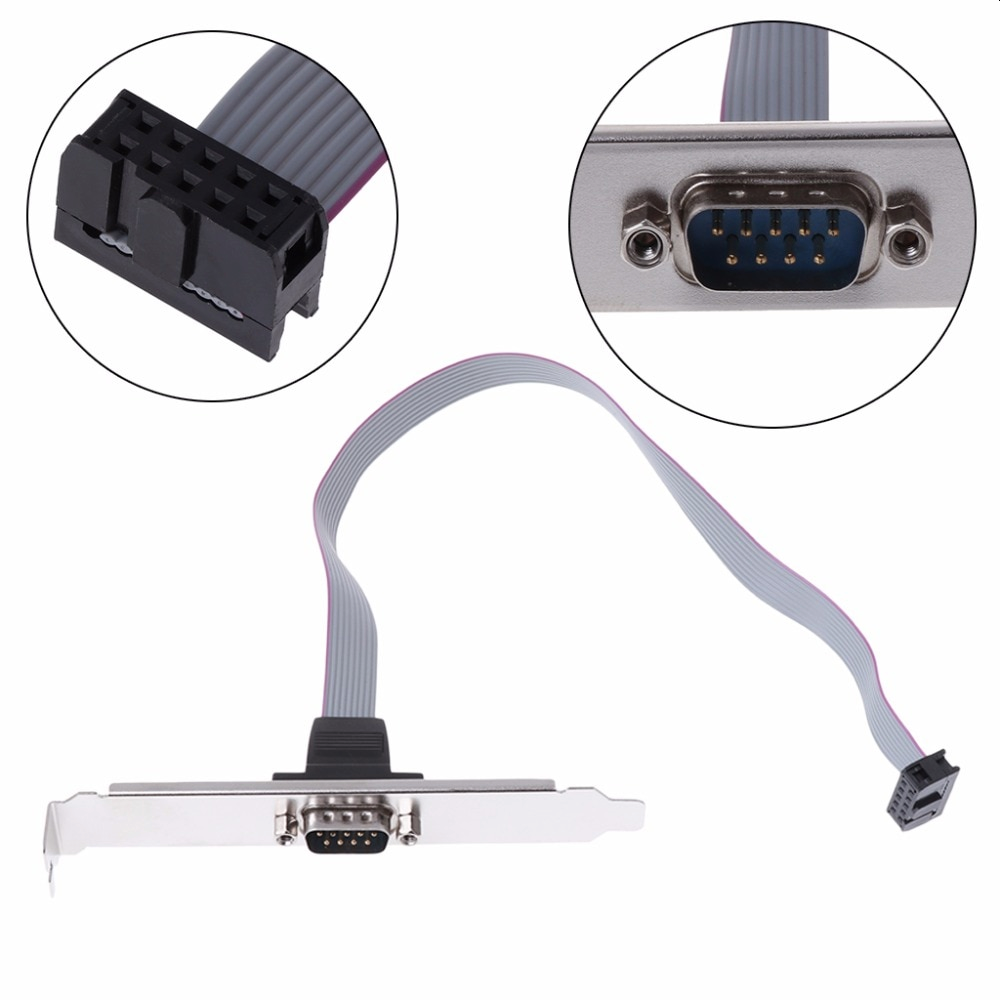
\includegraphics[width=0.9\linewidth]{images/joystick-pmod-thechief.png}
  \end{center}

\begin{minipage}{\linewidth}
\begin{center}
  \begin{longtable}{|L{3cm}|L{3cm}|p{3cm}|}
    \hline
    {\textbf{Joystick-actie}} & {\textbf{PMOD-JA-aansluitingen}} & {\textbf{DB9-aansluitingen}} \\
    \hline
    {Vuur} & {jahi(9)} & {pin 6} \\
    \hline
    {Omhoog} & {jalo(1)} & {pin 1} \\
    \hline
    {Links} & {jalo(2)} & {pin 3} \\
    \hline
    {Omlaag} & {jahi(7)} & {pin 2} \\
    \hline
    {Rechts} & {jahi(8)} & {pin 4} \\
    \hline
  \end{longtable}
\end{center}
\end{minipage}


\section{Handige tips}

Hier volgen enkele handige tips om vertrouwd te raken met de MEGA65:

\begin{itemize}

\item{Druk op \& houd \megasymbolkey (of de Commodore-toets als u een Commodore 64- of 65-toetsenbord gebruikt) ingedrukt tijdens het opstarten om in C64-modus op te starten in plaats van C65-modus.}
 \item{Druk op \& houd \specialkey{RUN\\STOP} ingedrukt tijdens het opstarten om de machine-taalmonitor te openen in plaats van BASIC te starten.}
\item{Druk op \widekey{RESTORE} en houd deze ongeveer een halve tot een seconde ingedrukt om het MEGA65 Freeze-menu te openen. Dit menu biedt handige hulpmiddelen om de processorsnelheid te wijzigen, te wisselen tussen PAL \& NTSC-videomodus, audio-instellingen aan te passen, freeze-states te beheren en D81-schijfimages te selecteren. U kunt bovendien het geheugen van het bevroren programma inspecteren en bewerken, en nog veel meer. Dit menu is in vele opzichten het hart van de MEGA65 en is het ontdekken zeker waard.}
\item{Typ \screentext{POKE0,65} in C64-modus om de processor op volle snelheid (40 MHz) te zetten. Sommige software gedraagt zich in deze modus onjuist, terwijl andere software juist sneller werkt.}
\item{Typ \screentext{POKE0,64} in C64-modus om de processor op 1 MHz te zetten.}
\item{Typ \screentext{SYS58552} in C64-modus om naar C65-modus te schakelen.}
\item{Typ \screentext{GO64} in C65-modus en bevestig door \screentext{Y} in te drukken om naar C64-modus te schakelen, hetzelfde als op een C128.}
\item{De C65-ROM maakt apparaat 8 tot standaard, zodat u het \textbf{,8} aan het einde van LOAD- en SAVE-commando's normaal gesproken kunt weglaten.}
\item{Het indrukken van \specialkey{SHIFT} + \specialkey{RUN\\STOP} in de C64- of C65-modus probeert van schijf op te starten.}
\end{itemize}

Veel plezier! Veel plezier! Er is jarenlang met liefde aan de MEGA65 gewerkt voor uw plezier. Wij hopen dat u er net zoveel plezier aan beleeft als wij bij het maken hebben gehad!

Het MEGA Museum of Electronic Games \& Art verwelkomt uw feedback, suggesties en bijdragen aan dit open-source-project voor het bewaren van digitaal erfgoed.
